\title{Data Acquisition System using an FSMD Circuit}
\date{}
\author{
	\IEEEauthorblockN{Daniel Josué Rodríguez Agraz}
	\IEEEauthorblockA{
		\textit{Communications and Electronics Enginnering, Unniversidad de Guadalajara}\\
	}
}

\documentclass[conference]{IEEEtran}
\def\endthebibliography{%
	\def\@noitemerr{\@latex@warning{Empty `thebibliography' environment}}%
	\endlist
}
\usepackage{filecontents,lipsum}
\usepackage[noadjust]{cite}
\usepackage{graphicx}
\usepackage{footmisc}
\usepackage{listings}
\usepackage{subcaption}
\usepackage{fancyhdr}
\usepackage{url}
\usepackage{hyperref}
\usepackage{array}
\usepackage{float}
\usepackage{adjustbox}
\usepackage{subcaption}
\hypersetup{
	colorlinks=true,
	linkcolor=black,
	urlcolor=blue,
	citecolor=black
}

\begin{document}
	
	\maketitle
	\begin{abstract}
    This document outlines the design and verification process of a data acquisition system (DAQ) using SystemVerilog. The DAQ system incorporates an Analog-to-Digital Converter (ADC), a 32x256 memory unit for data storage, an 8-bit address counter to manage memory write operations, and a state machine to orchestrate the interaction between these modules. The design and verification were conducted using the SystemVerilog hardware description language, with simulation and compilation performed in Questasim software. The design implementation follows a state machine approach. Additionally, a test bench was developed to verify each instance and the overall design, demonstrating the successful implementation of the circuit.

	This document focuses on the design and application of state machines and their significance in the digital design industry, where they are a critical tool for implementing control logic. State machines provide a structured way to describe the behavior of a system with a finite number of states and the transitions between them, ensuring efficient control of operational flow.

	\end{abstract}
	
	\section{Objectives}	
	\begin{itemize}
		\item Use Verilog to design and simulate a data acquisition system.
		\item Implement a finite state machine for circuit design.
		\item Design a test bench for the circuit verification.
	\end{itemize}
	
	\section{Introduction}
	A state machine is a logical system that progresses through a sequence of states defined by internal logic and external inputs.\cite{floyd_fundamentos_nodate} Sequential systems typically consist of inputs, outputs, and internal states. Two primary models are used to classify sequential circuits: the Mealy model and the Moore model.\cite{mano_digital_2002}
	
	\textbf{Mealy Model:} In a Mealy state machine, the outputs depend on both the current state and the current inputs. This model often results in faster response times, as changes in inputs can immediately affect the outputs without waiting for a state transition.\cite{mano_digital_2002}
	
	\textbf{Moore Model:} In a Moore state machine, the outputs depend solely on the current state and not directly on the inputs. As a result, the outputs only change on state transitions, which makes the design simpler and more predictable, though potentially slower to respond to input changes.\cite{mano_digital_2002}
	
	The Figure \ref{fig:sad-module} shows a diagram of the Data Acquisition System (SAD) module that will be implemented. The design of the Sample/Hold module and the ADC will be omitted, as they are outside the scope of this project. The state machine will control the storage of the data coming from the ADC module. Every time the ADC completes a conversion, the finite state machine (FSM) will enable the memory for the result to be stored, then increment the counter to set the next address for the subsequent data.
	
    \begin{figure}[H]
		\centering
		\includegraphics[width=0.9\columnwidth]{"Files/SAD Module"}
		\caption{}
		\label{fig:sad-module}
	\end{figure}
	
	In this project, a Mealy state machine is implemented to ensure proper data flow from the ADC to the memory. A crucial aspect of state machines is the state diagram, which illustrates state transitions based on inputs. As shown in Figure \ref{fig:state-diagram}, the next state is determined by the current state and the inputs, which act as conditionals to control transitions between states. For instance, in the transition from the sixth state to the seventh state, the value of the FAC input plays a critical role.
	
	\begin{figure}
		\centering
		\includegraphics[width=0.9\columnwidth]{"Files/State diagram"}
		\caption{State diagram for a FSM Data acquisition system.}
		\label{fig:state-diagram}
	\end{figure}
	
	\section{Methodology}
	For the design we will implement a Questasim project and will use systemVerilog languaje to achieve the design and verification.
	
	The first step involves implementing a memory module and a counter. In Verilog, a memory module can be created by defining a table of registers with the desired specifications. In this case, we will design a $32×256-bit$ memory.
	
	The memory operation is controlled by an enable input. When this input is set high, the system can perform either a write or read operation based on the state of the 
	$WR$ input. When the $WR$ input is low, reading is enabled, and the output will reflect the data stored at the address specified by the input address. Conversely, when the $WR$ input is high, the data present at the $data_in$ input will be stored in the specified memory address.
	
	To manage the memory and prevent overflow, as well as to generate a signal indicating to the state machine when the memory is full, a counter will be implemented. This counter will sequentially point to the corresponding address in the memory and will increment after each write operation. Once the counter reaches its maximum value, an overflow flag will be activated to inform the state machine that the memory is full.
	
	The data to be stored in the memory will come from an ADC module, the design of which is outside the scope of this project and will be omitted. Its corresponding signals will be emulated in the test bench.
	
	With these modules tested and operational, the next step is to design the state machine. For this, we will use the state diagram shown in Figure \ref{fig:state-diagram}. This diagram contains seven states divided into three stages.
	
	
   The first stage is initialization. After a reset, all outputs will be set to zero. Once the circuit receives a pulse on the $init$ signal, it will initialize the entire system. 
   
   First, the counter will be set to zero to avoid starting from a different address. Then, the start conversion signal will send a pulse to the ADC to begin sampling. While the ADC is busy, the state machine will be in standby mode. Once the ADC finishes the conversion, it will set the end-of-conversion (EOC) flag high, which will initiate the storage stage.
   
   In this stage, the memory will be enabled and set to write using the $en$ and $WR$ outputs. After saving the data, the counter will increment and point to the next memory address. This process will continue until the memory is full, at which point the full address flag will be set. Finally, the system will set the $ack$ high and will be waiting for the init signal to start again.
	
	\section{Results}
	
	The FIgure \ref{fig:first-reset-state} shows the states after a reset. It can be noticed that after a reset we send an initialization pulse. When the rising edge of the init enters, the counter reset output is set to high to restart the counter, which can be observed because just after that it is set to zero. After resetting the counter, we send the signal to the ADC to start the conversion, which lasts 11 cycles; during that time, we can se the waiting flag is set high, this signal was added to have a stand by state, which makes the design of the state machine easier. Once we receive the end of conversion pulse, the memory is enabled and the data is written, which can be seen in the data in signal, then the counter is incremented and the start conversion signal is set high for a new conversio, which can be seen in the Figure \ref{fig:second-saved-data}.
	\begin{figure}[H]
		\centering
		\includegraphics[width=\columnwidth]{"Files/First reset state"}
		\caption{}
		\label{fig:first-reset-state}
	\end{figure}

	
	\begin{figure}[H]
		\centering
		\includegraphics[width=\columnwidth]{"Files/second saved data"}
		\caption{Second and third readings.}
		\label{fig:second-saved-data}
	\end{figure}
	
	In the Figure \ref{fig:fillingmem} is shown how the memory starts gradually filling after the writing is enabled.
	
	\begin{figure}[H]
		\centering
		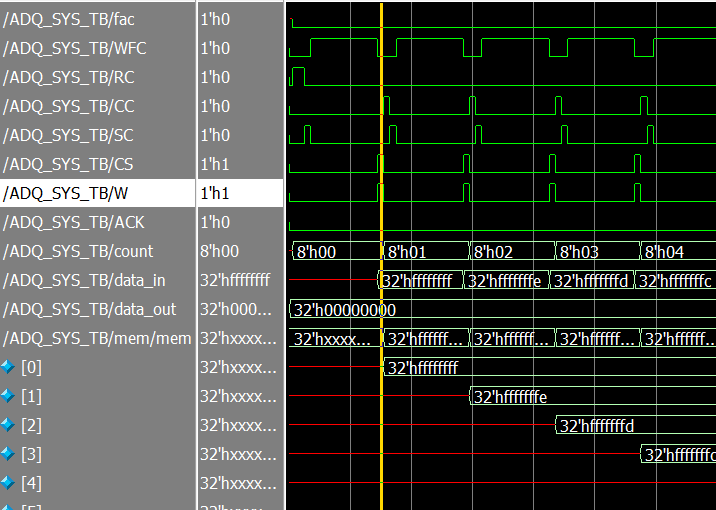
\includegraphics[width=\columnwidth]{Files/Filling_mem}
		\caption{}
		\label{fig:fillingmem}
	\end{figure}
	
	\begin{figure}[H]
		\centering
		\includegraphics[width=\columnwidth]{"Files/Counter reset"}
		\caption{}
		\label{fig:counter-reset}
	\end{figure}
	
	In the Figure \ref{fig:counter-reset-ack} once the counter is full, the ack signal is set to high, and doesnt change until a reset signal or an init sinal activate it.
	
	\begin{figure}[H]
		\centering
		\includegraphics[width=\columnwidth]{"Files/counter reset ack"}
		\caption{}
		\label{fig:counter-reset-ack}
	\end{figure}
	
	
	For the test bench a loop was used to go over every memory address, so by the end of the verification we can make sure the memory is filling up adequately. The data being saved is the subtraction of $'hFFFFFFFF$ and the variable being used in the loop.
	The Figure \ref{} shows the state of the memory at the end of the verification. 
	
	\begin{figure}[H]
		\centering
		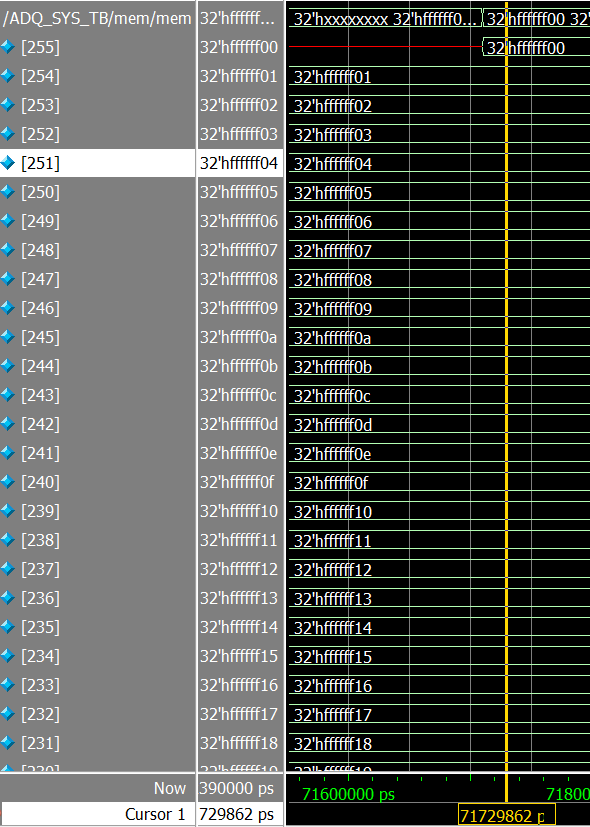
\includegraphics[width=\columnwidth]{Files/full_mem_val}
		\caption{}
		\label{fig:fullmemval}
	\end{figure}
	
	\begin{figure}[H]
		\centering
		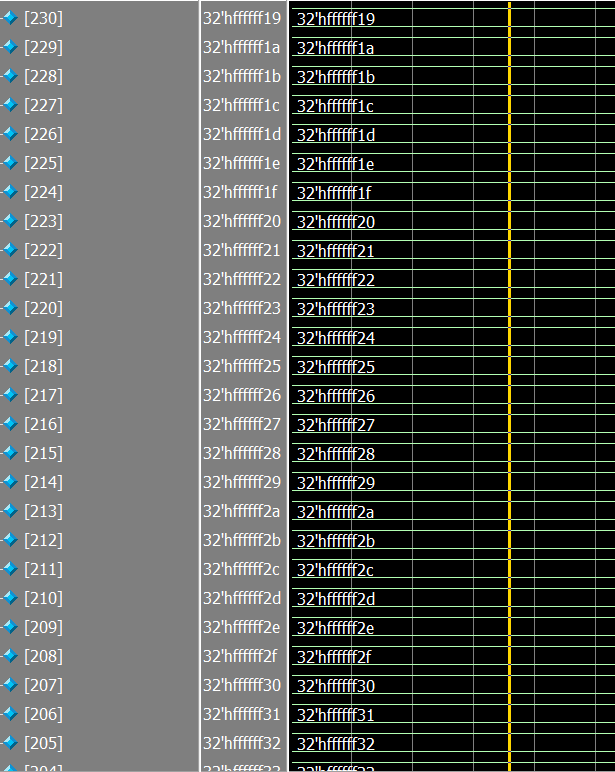
\includegraphics[width=\columnwidth]{Files/full_mem_val1}
		\caption{}
		\label{fig:fullmemval1}
	\end{figure}
	
	\begin{figure}[H]
		\centering
		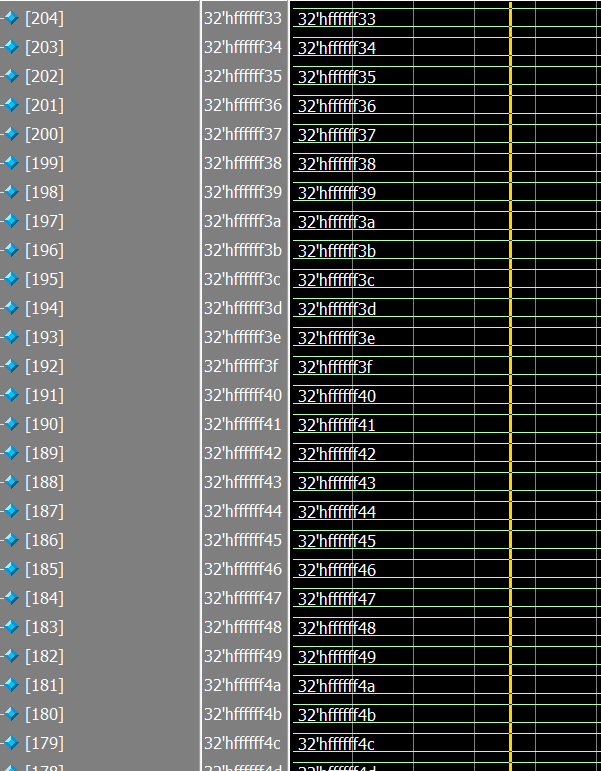
\includegraphics[width=\columnwidth]{Files/full_mem_val2}
		\caption{}
		\label{fig:fullmemval2}
	\end{figure}
	
	\begin{figure}[H]
		\centering
		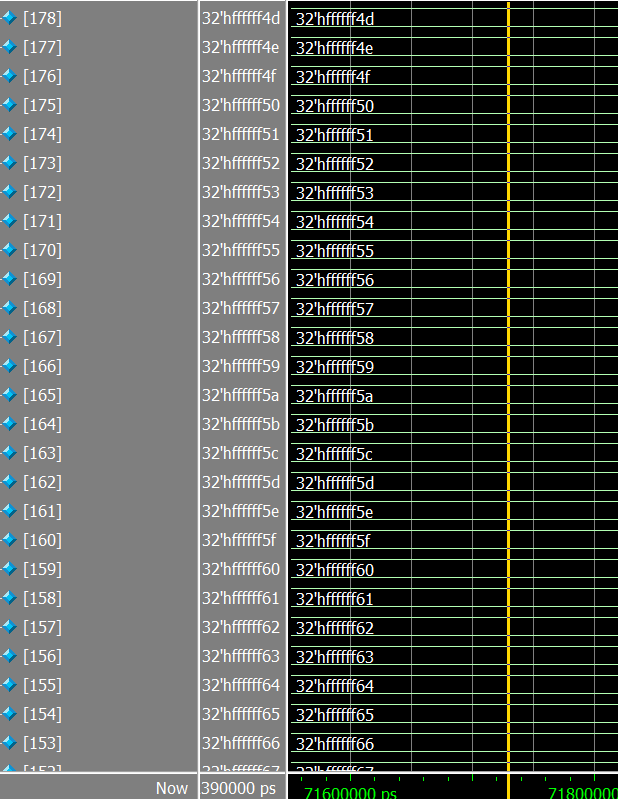
\includegraphics[width=\columnwidth]{Files/full_mem_val3}
		\caption{}
		\label{fig:fullmemval3}
	\end{figure}
	
	\begin{figure}[H]
		\centering
		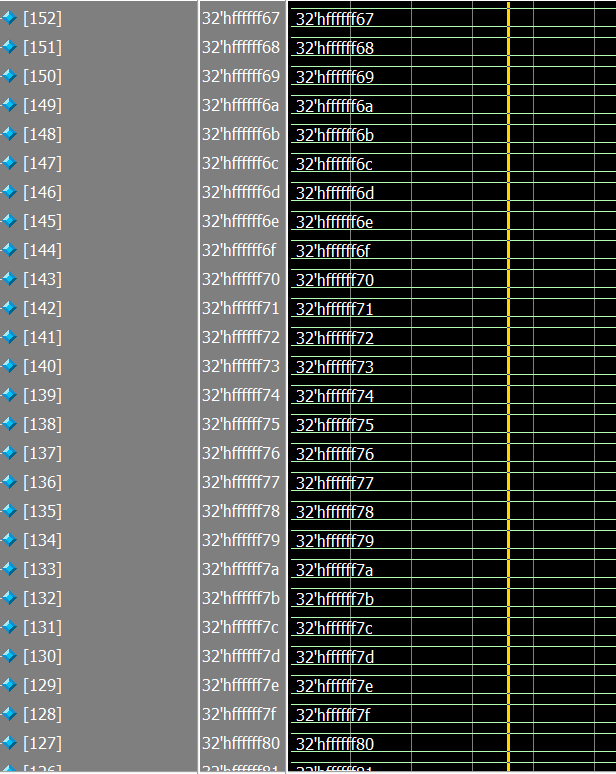
\includegraphics[width=\columnwidth]{Files/full_mem_val4}
		\caption{}
		\label{fig:fullmemval4}
	\end{figure}
	
	\begin{figure}[H]
		\centering
		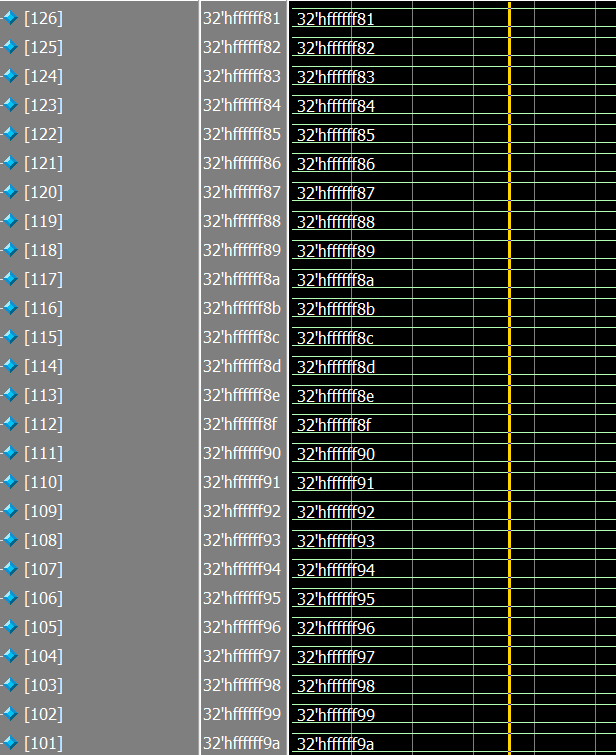
\includegraphics[width=\columnwidth]{Files/full_mem_val5}
		\caption{}
		\label{fig:fullmemval5}
	\end{figure}
	
	\begin{figure}[H]
		\centering
		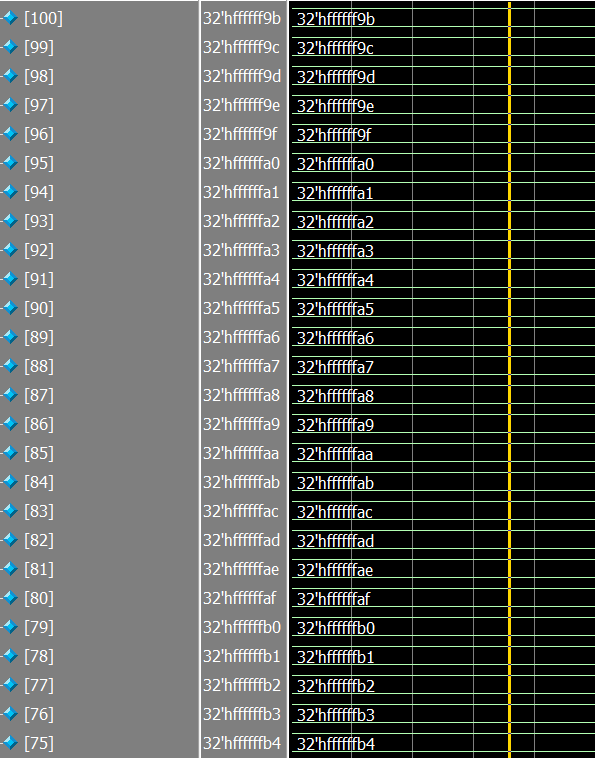
\includegraphics[width=\columnwidth]{Files/full_mem_val6}
		\caption{}
		\label{fig:fullmemval6}
	\end{figure}
	
	\begin{figure}[H]
		\centering
		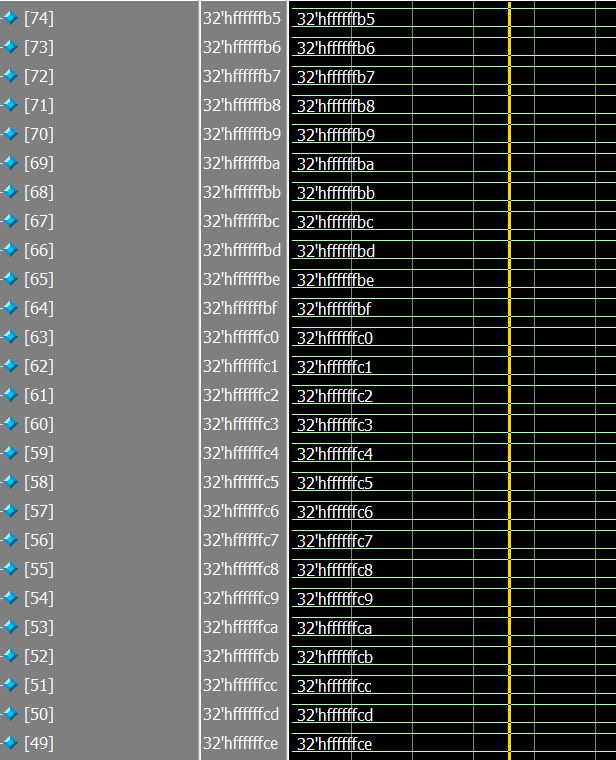
\includegraphics[width=\columnwidth]{Files/full_mem_val7}
		\caption{}
		\label{fig:fullmemval7}
	\end{figure}
	
	\begin{figure}[H]
		\centering
		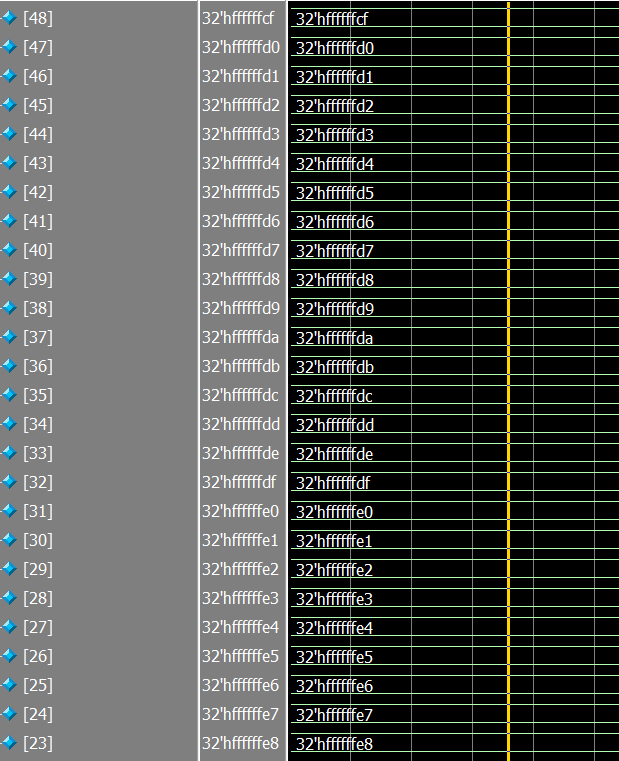
\includegraphics[width=\columnwidth]{Files/full_mem_val8}
		\caption{}
		\label{fig:fullmemval8}
	\end{figure}
	
	\begin{figure}[H]
		\centering
		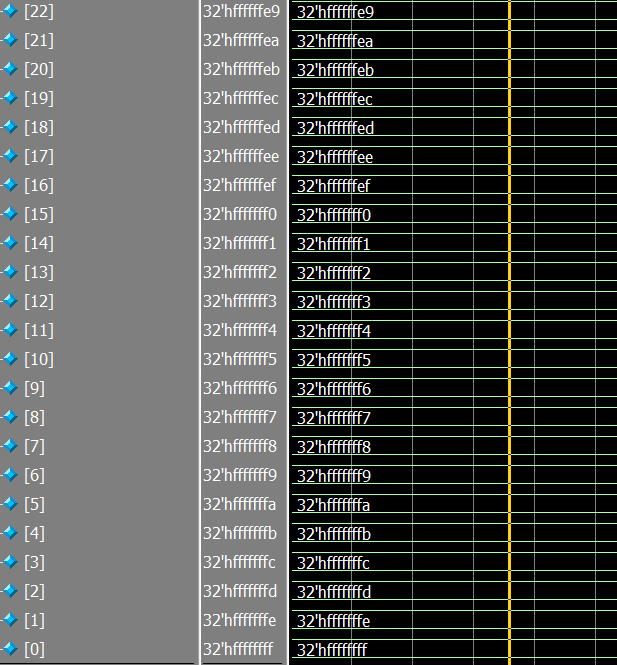
\includegraphics[width=\columnwidth]{Files/full_mem_val9}
		\caption{}
		\label{fig:fullmemval9}
	\end{figure}
	
	
	\section{Conclusions}
	
	Through this project, we successfully designed and implemented a data acquisition system using the SystemVerilog hardware description language. The design leveraged a state machine to control the data flow from an ADC circuit to a memory unit, where the ADC results were stored. Once the memory was full, an acknowledge signal was activated, prompting the system to wait for a reset before restarting. The project also included the successful design and verification of an 8-bit counter and a 32x256 memory.
	
	The state machine, crucial to managing the overall system flow, was implemented and tested alongside the memory and counter modules. In the test bench, these three modules were interconnected and thoroughly verified through simulations using Questasim, ensuring correct operation under various conditions.
	
	This approach, coupled with the implementation of a comprehensive testbench, demonstrated the effectiveness and reliability of the design.
	
	
	
	
	\bibliographystyle{IEEEtran}
	\bibliography{References}
	
	
	
	
	
	
\end{document}
